% ---------------------------------------------------------------------------
% Quelle der Abbildung:
%   Skript:  thesis/figures/scripts/hologramm_simulation.py (eigene Fresnel-Simulation,
%            N = 512, Padding 2, kein Trainingslauf, kein HoloForge-Datensatz)
%   Aufruf:  /tmp/holo311/bin/python thesis/figures/scripts/hologramm_simulation.py
%   Basis:   Commit 1abccf9 (Branch cursor/thesis-grundlagen-6175), 2026-10-01
%   Dateien: hologramm_spektrum.pdf (dieses Skript erzeugt außerdem
%            figures/stand_der_technik/radialprofil_spektrum.pdf)
% Einbinden im Kapitel: % ---------------------------------------------------------------------------
% Quelle der Abbildung:
%   Skript:  thesis/figures/scripts/hologramm_simulation.py (eigene Fresnel-Simulation,
%            N = 512, Padding 2, kein Trainingslauf, kein HoloForge-Datensatz)
%   Aufruf:  /tmp/holo311/bin/python thesis/figures/scripts/hologramm_simulation.py
%   Basis:   Commit 1abccf9 (Branch cursor/thesis-grundlagen-6175), 2026-10-01
%   Dateien: hologramm_spektrum.pdf (dieses Skript erzeugt außerdem
%            figures/stand_der_technik/radialprofil_spektrum.pdf)
% Einbinden im Kapitel: % ---------------------------------------------------------------------------
% Quelle der Abbildung:
%   Skript:  thesis/figures/scripts/hologramm_simulation.py (eigene Fresnel-Simulation,
%            N = 512, Padding 2, kein Trainingslauf, kein HoloForge-Datensatz)
%   Aufruf:  /tmp/holo311/bin/python thesis/figures/scripts/hologramm_simulation.py
%   Basis:   Commit 1abccf9 (Branch cursor/thesis-grundlagen-6175), 2026-10-01
%   Dateien: hologramm_spektrum.pdf (dieses Skript erzeugt außerdem
%            figures/stand_der_technik/radialprofil_spektrum.pdf)
% Einbinden im Kapitel: % ---------------------------------------------------------------------------
% Quelle der Abbildung:
%   Skript:  thesis/figures/scripts/hologramm_simulation.py (eigene Fresnel-Simulation,
%            N = 512, Padding 2, kein Trainingslauf, kein HoloForge-Datensatz)
%   Aufruf:  /tmp/holo311/bin/python thesis/figures/scripts/hologramm_simulation.py
%   Basis:   Commit 1abccf9 (Branch cursor/thesis-grundlagen-6175), 2026-10-01
%   Dateien: hologramm_spektrum.pdf (dieses Skript erzeugt außerdem
%            figures/stand_der_technik/radialprofil_spektrum.pdf)
% Einbinden im Kapitel: \input{figures/grundlagen/hologramm_spektrum}
% ---------------------------------------------------------------------------
\begin{figure}[!tb]
  \centering
  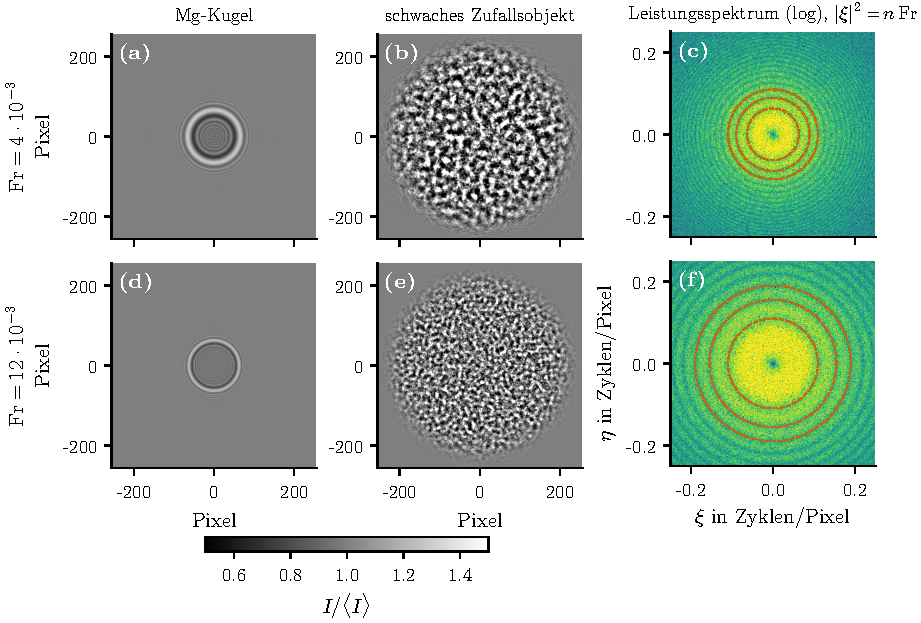
\includegraphics[width=\textwidth]{figures/grundlagen/hologramm_spektrum}
  \caption[Simulierte Hologramme und Leistungsspektren bei zwei Fresnel-Zahlen]{%
    Simulierte Hologramme nach \cref{eq:grundlagen:propagation} bei
    $\Fr = \num{4e-3}$ (obere Zeile) und $\Fr = \num{1.2e-2}$ (untere Zeile)
    auf einem Ausschnitt von $512\times512$ Pixeln (Rechengitter $1024^2$,
    sodass $N \geq 1/\Fr$ erfüllt ist). (a,\,d)~Magnesiumkugel mit
    \qty{9}{\micro\metre} Durchmesser bei \qty{11}{\kilo\electronvolt}
    (Phasenschub im Zentrum \qty{-1.5}{\radian}, Absorption \qty{2.5}{\percent}):
    Je kleiner $\Fr$, desto weiter reichen die Fresnel-Säume über den
    geometrischen Schatten hinaus. (b,\,e)~Schwaches reines Phasenobjekt mit
    glatter Zufallstextur (Standardabweichung der Phase \qty{0.3}{\radian}).
    (c,\,f)~Logarithmisches Leistungsspektrum $\abs{\mathcal{F}[I/\langle I\rangle - 1]}^2$
    des Zufallsobjekts; die gestrichelten Kreise markieren $\xi^2+\eta^2 = n\,\Fr$
    für $n = 1,2,3$, die Nullstellen des Phasenkontrasts nach
    \cref{eq:grundlagen:ctf}. Die beiden Fresnel-Zahlen entsprechen in der um
    den Faktor~8 gebinnten P05-Geometrie ($\dx = \qty{52}{\micro\metre}$,
    $\zTwo = \qty{20}{\metre}$) etwa $\zOne \approx \qty{67}{\milli\metre}$ bzw.\
    \qty{198}{\milli\metre}.}
  \label{fig:grundlagen:hologramm}
\end{figure}

% ---------------------------------------------------------------------------
\begin{figure}[!tb]
  \centering
  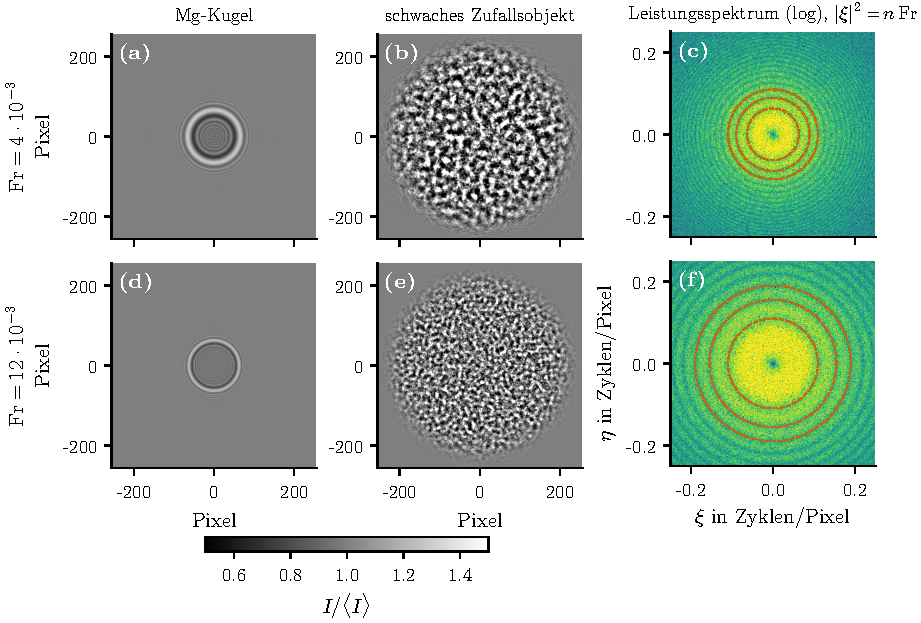
\includegraphics[width=\textwidth]{figures/grundlagen/hologramm_spektrum}
  \caption[Simulierte Hologramme und Leistungsspektren bei zwei Fresnel-Zahlen]{%
    Simulierte Hologramme nach \cref{eq:grundlagen:propagation} bei
    $\Fr = \num{4e-3}$ (obere Zeile) und $\Fr = \num{1.2e-2}$ (untere Zeile)
    auf einem Ausschnitt von $512\times512$ Pixeln (Rechengitter $1024^2$,
    sodass $N \geq 1/\Fr$ erfüllt ist). (a,\,d)~Magnesiumkugel mit
    \qty{9}{\micro\metre} Durchmesser bei \qty{11}{\kilo\electronvolt}
    (Phasenschub im Zentrum \qty{-1.5}{\radian}, Absorption \qty{2.5}{\percent}):
    Je kleiner $\Fr$, desto weiter reichen die Fresnel-Säume über den
    geometrischen Schatten hinaus. (b,\,e)~Schwaches reines Phasenobjekt mit
    glatter Zufallstextur (Standardabweichung der Phase \qty{0.3}{\radian}).
    (c,\,f)~Logarithmisches Leistungsspektrum $\abs{\mathcal{F}[I/\langle I\rangle - 1]}^2$
    des Zufallsobjekts; die gestrichelten Kreise markieren $\xi^2+\eta^2 = n\,\Fr$
    für $n = 1,2,3$, die Nullstellen des Phasenkontrasts nach
    \cref{eq:grundlagen:ctf}. Die beiden Fresnel-Zahlen entsprechen in der um
    den Faktor~8 gebinnten P05-Geometrie ($\dx = \qty{52}{\micro\metre}$,
    $\zTwo = \qty{20}{\metre}$) etwa $\zOne \approx \qty{67}{\milli\metre}$ bzw.\
    \qty{198}{\milli\metre}.}
  \label{fig:grundlagen:hologramm}
\end{figure}

% ---------------------------------------------------------------------------
\begin{figure}[!tb]
  \centering
  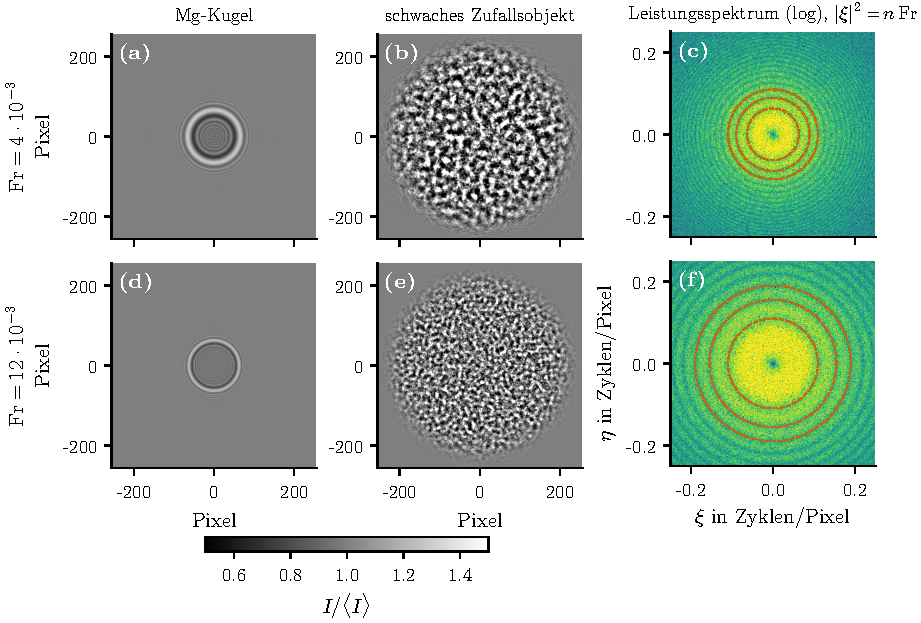
\includegraphics[width=\textwidth]{figures/grundlagen/hologramm_spektrum}
  \caption[Simulierte Hologramme und Leistungsspektren bei zwei Fresnel-Zahlen]{%
    Simulierte Hologramme nach \cref{eq:grundlagen:propagation} bei
    $\Fr = \num{4e-3}$ (obere Zeile) und $\Fr = \num{1.2e-2}$ (untere Zeile)
    auf einem Ausschnitt von $512\times512$ Pixeln (Rechengitter $1024^2$,
    sodass $N \geq 1/\Fr$ erfüllt ist). (a,\,d)~Magnesiumkugel mit
    \qty{9}{\micro\metre} Durchmesser bei \qty{11}{\kilo\electronvolt}
    (Phasenschub im Zentrum \qty{-1.5}{\radian}, Absorption \qty{2.5}{\percent}):
    Je kleiner $\Fr$, desto weiter reichen die Fresnel-Säume über den
    geometrischen Schatten hinaus. (b,\,e)~Schwaches reines Phasenobjekt mit
    glatter Zufallstextur (Standardabweichung der Phase \qty{0.3}{\radian}).
    (c,\,f)~Logarithmisches Leistungsspektrum $\abs{\mathcal{F}[I/\langle I\rangle - 1]}^2$
    des Zufallsobjekts; die gestrichelten Kreise markieren $\xi^2+\eta^2 = n\,\Fr$
    für $n = 1,2,3$, die Nullstellen des Phasenkontrasts nach
    \cref{eq:grundlagen:ctf}. Die beiden Fresnel-Zahlen entsprechen in der um
    den Faktor~8 gebinnten P05-Geometrie ($\dx = \qty{52}{\micro\metre}$,
    $\zTwo = \qty{20}{\metre}$) etwa $\zOne \approx \qty{67}{\milli\metre}$ bzw.\
    \qty{198}{\milli\metre}.}
  \label{fig:grundlagen:hologramm}
\end{figure}

% ---------------------------------------------------------------------------
\begin{figure}[!tb]
  \centering
  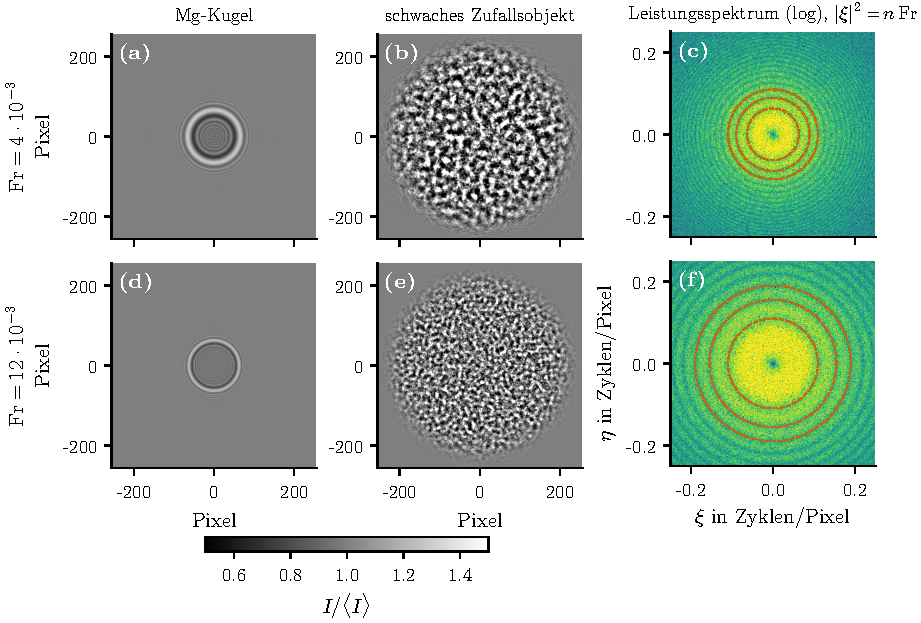
\includegraphics[width=\textwidth]{figures/grundlagen/hologramm_spektrum}
  \caption[Simulierte Hologramme und Leistungsspektren bei zwei Fresnel-Zahlen]{%
    Simulierte Hologramme nach \cref{eq:grundlagen:propagation} bei
    $\Fr = \num{4e-3}$ (obere Zeile) und $\Fr = \num{1.2e-2}$ (untere Zeile)
    auf einem Ausschnitt von $512\times512$ Pixeln (Rechengitter $1024^2$,
    sodass $N \geq 1/\Fr$ erfüllt ist). (a,\,d)~Magnesiumkugel mit
    \qty{9}{\micro\metre} Durchmesser bei \qty{11}{\kilo\electronvolt}
    (Phasenschub im Zentrum \qty{-1.5}{\radian}, Absorption \qty{2.5}{\percent}):
    Je kleiner $\Fr$, desto weiter reichen die Fresnel-Säume über den
    geometrischen Schatten hinaus. (b,\,e)~Schwaches reines Phasenobjekt mit
    glatter Zufallstextur (Standardabweichung der Phase \qty{0.3}{\radian}).
    (c,\,f)~Logarithmisches Leistungsspektrum $\abs{\mathcal{F}[I/\langle I\rangle - 1]}^2$
    des Zufallsobjekts; die gestrichelten Kreise markieren $\xi^2+\eta^2 = n\,\Fr$
    für $n = 1,2,3$, die Nullstellen des Phasenkontrasts nach
    \cref{eq:grundlagen:ctf}. Die beiden Fresnel-Zahlen entsprechen in der um
    den Faktor~8 gebinnten P05-Geometrie ($\dx = \qty{52}{\micro\metre}$,
    $\zTwo = \qty{20}{\metre}$) etwa $\zOne \approx \qty{67}{\milli\metre}$ bzw.\
    \qty{198}{\milli\metre}.}
  \label{fig:grundlagen:hologramm}
\end{figure}
